\documentclass[tikz,border=5pt]{standalone}
\usepackage[T1]{fontenc}
\usepackage{lmodern,amsmath,amssymb}
\usetikzlibrary{arrows.meta,calc,positioning,fit,backgrounds,shapes.geometric,matrix,decorations.pathreplacing,patterns}
\definecolor{ink}{gray}{0.08}
\definecolor{wash}{gray}{0.965}
\definecolor{soft}{gray}{0.45}
\tikzset{box/.style={draw=ink,line width=.65pt,fill=white,align=center,inner sep=4pt,outer sep=0pt,font=\small},flow/.style={draw=ink,line width=.65pt,-{Latex[length=1.8mm,width=1.3mm]},rounded corners=2pt},annotation/.style={font=\scriptsize,text=soft,align=center},groupbox/.style={draw=soft,dashed,line width=.45pt,fill=wash}}
\begin{document}
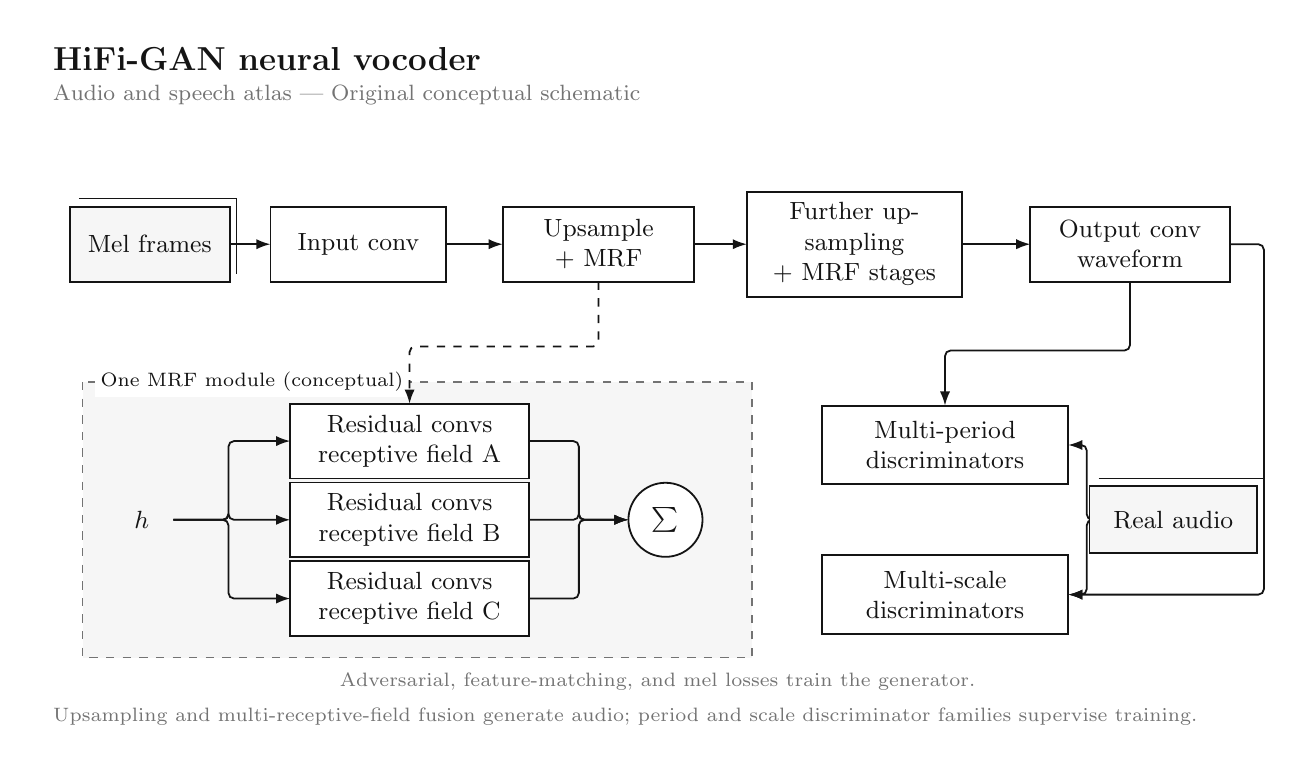
\begin{tikzpicture}[x=1cm,y=-1cm,font=\rmfamily,text=ink]

\path[use as bounding box] (0,0) rectangle (16,9);
\node[anchor=west,font=\large\bfseries] at (.2,.4) {HiFi-GAN neural vocoder};
\node[anchor=west,font=\footnotesize,text=soft] at (.2,.85) {Audio and speech atlas | Original conceptual schematic};
\begin{pgfonlayer}{background}
\draw[groupbox] (0.7,4.5) rectangle (9.2,8.0);
\node[anchor=west,font=\scriptsize,fill=white,inner sep=2pt] at (0.85,4.5) {One MRF module (conceptual)};
\end{pgfonlayer}
\node[box,fill=wash,minimum width=2.0cm,minimum height=0.95cm,text width=1.75cm] (mel) at (1.55,2.75) {Mel frames};
\draw[ink,line width=.4pt] (0.65,2.175) -- (2.65,2.175) -- (2.65,3.125);
\node[box,minimum width=2.2cm,minimum height=0.95cm,text width=1.9500000000000002cm] (pre) at (4.2,2.75) {Input conv};
\node[box,minimum width=2.4cm,minimum height=0.95cm,text width=2.15cm] (up1) at (7.25,2.75) {Upsample\\+ MRF};
\node[box,minimum width=2.7cm,minimum height=0.95cm,text width=2.45cm] (up2) at (10.5,2.75) {Further upsampling\\+ MRF stages};
\node[box,minimum width=2.5cm,minimum height=0.95cm,text width=2.25cm] (wave) at (14.0,2.75) {Output conv\\waveform};
\node[align=center,inner sep=0pt,outer sep=0pt,font=\small,minimum width=0.8cm,minimum height=0.6cm,text width=0.55cm] (mrfIn) at (1.45,6.25) {$h$};
\node[box,minimum width=3.0cm,minimum height=0.75cm,text width=2.75cm] (ra) at (4.85,5.25) {Residual convs\\receptive field A};
\node[box,minimum width=3.0cm,minimum height=0.75cm,text width=2.75cm] (rb) at (4.85,6.25) {Residual convs\\receptive field B};
\node[box,minimum width=3.0cm,minimum height=0.75cm,text width=2.75cm] (rc) at (4.85,7.25) {Residual convs\\receptive field C};
\node[box,circle,minimum width=0.7cm,minimum height=0.7cm,text width=0.44999999999999996cm] (mrfSum) at (8.1,6.25) {$\sum$};
\node[box,minimum width=3.1cm,minimum height=1.0cm,text width=2.85cm] (mpd) at (11.65,5.3) {Multi-period\\discriminators};
\node[box,minimum width=3.1cm,minimum height=1.0cm,text width=2.85cm] (msd) at (11.65,7.2) {Multi-scale\\discriminators};
\node[box,fill=wash,minimum width=2.1cm,minimum height=0.85cm,text width=1.85cm] (real) at (14.55,6.25) {Real audio};
\draw[ink,line width=.4pt] (13.6,5.7250000000000005) -- (15.700000000000001,5.7250000000000005) -- (15.700000000000001,6.575);
\begin{pgfonlayer}{background}
\draw[flow] (mel.east) -- (pre.west);
\draw[flow] (pre.east) -- (up1.west);
\draw[flow] (up1.east) -- (up2.west);
\draw[flow] (up2.east) -- (wave.west);
\draw[flow] (mrfIn.east) -- (2.55,6.25) -- (2.55,5.25) -- (ra.west);
\draw[flow] (mrfIn.east) -- (2.55,6.25) -- (2.55,6.25) -- (rb.west);
\draw[flow] (mrfIn.east) -- (2.55,6.25) -- (2.55,7.25) -- (rc.west);
\draw[flow] (ra.east) -- (7.0,5.25) -- (7.0,6.25) -- (mrfSum.west);
\draw[flow] (rb.east) -- (7.0,6.25) -- (7.0,6.25) -- (mrfSum.west);
\draw[flow] (rc.east) -- (7.0,7.25) -- (7.0,6.25) -- (mrfSum.west);
\draw[flow,dashed] (up1.south) -- (7.25,4.05) -- (4.85,4.05) -- (ra.north);
\draw[flow] (wave.south) -- (14,4.1) -- (11.65,4.1) -- (mpd.north);
\draw[flow] (wave.east) -- (15.7,2.75) -- (15.7,7.2) -- (msd.east);
\draw[flow] (real.west) -- (13.45,6.25) -- (13.45,5.3) -- (mpd.east);
\draw[flow] (real.west) -- (13.45,6.25) -- (13.45,7.2) -- (msd.east);
\end{pgfonlayer}
\node[align=center,anchor=center,font=\scriptsize,text=soft,text width=14cm] at (8,8.3) {Adversarial, feature-matching, and mel losses train the generator.};
\node[anchor=west,align=left,font=\scriptsize,text=soft,text width=15.6cm] at (.2,8.75) {Upsampling and multi-receptive-field fusion generate audio; period and scale discriminator families supervise training.};
\end{tikzpicture}
\end{document}
